\documentclass[12pt,a4paper,halfparskip]{scrartcl}
\usepackage[latin1]{inputenc}
\usepackage{graphicx}
\usepackage{xspace}
\usepackage{amsmath}
\usepackage{floatflt}
\usepackage{xcolor}
\usepackage[urlbordercolor={0 0 1},raiselinks,pagebackref]{hyperref}

\overfullrule 2mm
\title{Java Finite Automata\\---\\A Tutorial}
\author{Harald Kirsch\\\texttt{\small Harald.Kirsch@pifpafpuf.de}}

\newcommand{\monqjfa}{\texttt{monq.jfa}\xspace}
\newcommand{\monqjarlink}{\href{http://pifpafpuf.de/Monq.jfa/download}{\code{monq.jar}}\xspace}

\newcommand{\urlExamplebase}{http://pifpafpuf.de/Monq.jfa/download}
\newcommand{\hrefComptest}{\href{\urlExamplebase/CompileTest.java}{\code{CompileTest.java}}\xspace}
\newcommand{\hrefExample}{\href{\urlExamplebase/Example.java}{\code{Example.java}}\xspace}
\newcommand{\hrefExampleFaAction}{\href{\urlExamplebase/ExampleFaAction.java}{\code{ExampleFaAction.java}}\xspace}
\newcommand{\hrefPatConf}{\href{\urlExamplebase/PatternConflict.java}{\code{PatternConflict.java}}\xspace}
\newcommand{\hrefCountWords}{\href{\urlExamplebase/CountWords.java}{\code{CountWords.java}}\xspace}


\newcommand{\urlApibase}{http://pifpafpuf.de/Monq.jfa/monqApiDoc}
\newcommand{\urlResyntax}{\urlApibase/monq/jfa/doc-files/resyntax.html}
\newcommand{\urlCaptparen}{\urlApibase/monq/jfa/doc-files/resyntax.html\#rse}
\newcommand{\urlUnicats}{http://www.unicode.org/unicode/reports/tr18/\#Categories}
\newcommand{\urlShortest}{\urlApibase/monq/jfa/doc-files/resyntax.html\#greed}
\newcommand{\urlFriedl}{http://www.oreilly.com/catalog/regex/}
\newcommand{\urlFString}{\urlApibase/monq/jfa/PrintfFormatter.html}

\newcommand{\hrefActions}{\href{\urlApibase/monq/jfa/actions/package-summary.html}{\code{monq.jfa.actions}}\xspace}

\newcommand{\hrefDROP}{\href{\urlApibase/monq/jfa/DfaRun.html\#UNMATCHED_DROP}{\code{UNMATCHED\_DROP}}\xspace}
\newcommand{\hrefCOPY}{\href{\urlApibase/monq/jfa/DfaRun.html\#UNMATCHED_COPY}{\code{UNMATCHED\_COPY}}\xspace}
\newcommand{\hrefTHROW}{\href{\urlApibase/monq/jfa/DfaRun.html\#UNMATCHED_THROW}{\code{UNMATCHED\_THROW}}\xspace}
\newcommand{\hrefDfaRun}{\href{\urlApibase/monq/jfa/DfaRun.html}{\code{DfaRun}}\xspace}
\newcommand{\hrefDfa}{\href{\urlApibase/monq/jfa/Dfa.html}{\code{Dfa}}\xspace}
\newcommand{\hrefCollect}{\href{\urlApibase/monq/jfa/DfaRun.html\#collect}{\code{DfaRun.collect}}\xspace}
\newcommand{\hrefClientdata}{\href{\urlApibase/monq/jfa/DfaRun.html\#clientData}{\code{DfaRun.clientData}}\xspace}

\newcommand{\hrefNfa}{\href{\urlApibase/monq/jfa/Nfa.html}{\code{Nfa}}\xspace}
\newcommand{\hrefFaAction}{\href{\urlApibase/monq/jfa/FaAction.html}{\code{FaAction}}\xspace}
\newcommand{\hrefInvoke}{\href{\urlApibase/monq/jfa/FaAction.html\#invoke\%28java.lang.StringBuffer,\%20int,\%20monq.jfa.DfaRun\%29}{\code{FaAction.invoke()}}\xspace}
\newcommand{\hrefmergeWith}{\href{\urlApibase/monq/jfa/FaAction.html\#mergeWith\%28monq.jfa.FaAction\%29}{\code{FaAction.mergeWith()}}\xspace}
\newcommand{\hrefAbstractFaAction}{\href{\urlApibase/monq/jfa/AbstractFaAction.html}{\code{AbstractFaAction}}\xspace}
\newcommand{\hrefPrintf}{\href{\urlApibase/monq/jfa/actions/Printf.html}{\code{Printf}}\xspace}
\newcommand{\hrefCDE}{\href{\urlApibase/monq/jfa/CompileDfaException.html}{\code{CompileDfaException}}\xspace}

\newcommand{\hrefUniprot}{\href{http://www.uniprot.org}{\textsc{UniProt}}\xspace}



\newsavebox{\codebox}
\newenvironment{codexa}%
{\begin{lrbox}{\codebox}\begin{minipage}{0.85\textwidth}\small\tt}
{\end{minipage}\end{lrbox}\begin{center}\setlength{\fboxrule}{1pt}\setlength{\fboxsep}{1em}\fcolorbox{codexab}{codexa}{\usebox{\codebox}}\end{center}}


\definecolor{codexa}{HTML}{F0F0F0}
\definecolor{codexb}{HTML}{404080}
\definecolor{codexab}{HTML}{E0E0FF}

\newcommand{\code}[1]{\texttt{#1}}
\newcommand{\T}{\hspace*{2ex}}
%%%%%%%%%%%%%%%%%%%%%%%%%%%%%%%%%%%%%%%%%%%%%%%%%%%%%%%%%%%%%%%%%%%%%%%%
\begin{document}
\begin{titlepage}
  {\tiny \today}
  \vfill
  \begin{raggedleft}
   \Huge\tt monq.jfa\\
   \bf\sf Java Finite Automata\\
   A Tutorial\\
   \strut
  \end{raggedleft}

  \begin{raggedleft}
    \large
  Harald Kirsch\\
  \texttt{\small Harald.Kirsch@pifpafpuf.de}\\
  \strut
  \end{raggedleft}
  \vfill
  
\includegraphics{JfaLogo.png}\vspace*{-2cm}
\end{titlepage}
\newpage
\tableofcontents


%%%%%%%%%%%%%%%%%%%%%%%%%%%%%%%%%%%%%%%%%%%%%%%%%%%%%%%%%%%%%%%%%%%%%%%%

\section{Introduction}
Like with other Java class library, the intention and best use of
many classes of \texttt{monq.jfa} is not necessarily easy to grasp
from reading the API documentation alone.
A bit like with Lego$^{\text{TM}}$ bricks some uses are straight
forward, but efficient and effective use requires understanding and
creativity that can best be trained by example. This tutorial tries to
help you get started.

In order to see quickly whether \monqjfa is for you or whether
\texttt{java.util.regexp} is just enough, have a quick look at
section~\ref{sec:keyfeatures} about the key features.

This tutorial assumes that you are familiar with Java and that you
have used simple regular expressions in the past. Only the more tricky
features of regular expressions as available in \monqjfa will be
explained.



\section{Preparation}
\subsection{Download}
To be able to follow the tutorial, you should compile and run a
few simple example programs. To do so, you need access to the monq
class library:

\begin{enumerate}
\item Download \monqjarlink.
\item Make sure your Java virtual machine has access to
  \texttt{monq.jar} by adding it to the class path used.
\item Make sure you have access to a command line on which to start
  the sample programs we compile.
\end{enumerate}

\subsection{Check that it works}
To check whether you succeded in making \texttt{monq.jar} available in
your class path, please download \hrefComptest
or copy and paste the code
\begin{verbatim}
import monq.jfa.*;
public class CompileTest {
  public static Nfa nfa = new Nfa(Nfa.NOTHING);
}
\end{verbatim}


into a file with that name. Then compile it with your Java system. If
it compiles without error, you are most likely set up fine and
we can start with more interesting things.

\section{Summary of Lessons}
\begin{description}
\item[A First Example]  shows how to convert
  pieces of text according to a single pattern with an associated
  action (section \ref{sec:firstexa}).
\item[Conflicting Patterns] describes how to deal with cases where
  more than one pattern matches a piece of text. A decision has to be
  taken as to which action to run.
  (section~\ref{sec:confpats}).
\item[Implementing Actions] While there are a few general purpose
  actions provided already in \hrefActions, most non-trivial
  applications will require specialized actions to be implemented.
  This lesson describes the inner workings of actions
  (section~\ref{sec:actions}).
\item[Co-operating Actions] Apart from just converting one text into
  another, Jfa is perfectly suited to parse text and built up internal
  data structures. This lesson describes, how several actions can
  co-operate in a thread safe manner on filling an internal data
  structure (section~\ref{sec:coopActions}).
\item[Collect Mode] In this lesson you learn how to take control over
  when exactly the machinery writes processed text to the output. This
  allows actions to look back on already processed text. It is
  typically used to postpone the decision whether a piece of text
  shall be deleted or not. For example you can stop writing output at
  the beginning of line. At the end of the line the decision whether
  to write or delete it can be based on the matches found while
  processing the line (section~\ref{sec:collect}).
\item[Shortest Match] A feature not available in any other regular
  expression package is an operator to request the shortest match.
  Luckily there is no need to write up a lesson for it, because it is
  explained already well in the api documentation. See the section on
  \href{\urlShortest}{Non Greedy Matching vs.{} Shortest Match}.
\item[Thread Safe Dfa] discusses how to make sure that a Dfa can be
  shared between threads (section~\ref{sec:threadsafe}).
\item[Actions from Scratch] explains why and how you would implement
  an \hrefFaAction from scratch instead of extending
  \hrefAbstractFaAction (section~\ref{sec:actionFromScratch}).
\item[Coding Hints] gives some general hints of how to organise
  your code around a \code{Dfa} (section~\ref{sec:codeguide}).
\end{description}


\section{A First Example}\label{sec:firstexa}

Please download and compile the file \hrefExample.

As a first quick check that it works, run the following command line:


\begin{codexa}
\% echo 123 | java Example 2 x
\end{codexa}

You should see the output

\begin{codexa}
\% 1x3
\end{codexa}

Before we look at the code, lets try some more examples. The program takes two arguments. We will see later in the code that the first is a regular expression and the second is a format string that describes how any text matching the pattern shall be transformed. Try this

\begin{codexa}
\% echo hallo 123 hallo | java Example1 '[0-9]+' '=\%0='\\
hallo =123= hallo
\end{codexa}

The \href{\urlResyntax}{regular expression} \code{[0-9]+} is fairly
standard to match a sequence of digits. The \code{\%0} in the
\href{\urlFString}{format string} references the matching text.

Now lets look at the code. The crucial line achieving most of the
functionality of our program is this:

\begin{codexa}
  Nfa nfa = new Nfa(argv[0], new Printf(argv[1]));
\end{codexa}

An \hrefNfa is created that binds the regular expression
\code{argv[0]} to an action. The action is a \hrefPrintf object
that knows how to interprete the format passed as \code{argv[1]}. The
idea is that whenever a match for \code{argv[0]} is found, the action
is called to rewrite the matching text according to the action. In
most cases, an \code{Nfa} will not only contain just one
pattern/action pair, but many, as shown in the lesson on Conflicting
Patterns (section~\ref{sec:confpats}).

But what shall the machinery do with text that is not matched by any
pattern. Three possibilities are provided:

\begin{enumerate}
\item the text can be dropped (deleted) \hrefDROP
\item the text can be copied \hrefCOPY
\item the machinery can throw an exception \hrefTHROW.
\end{enumerate}

As seen from the output of the example program, it copies non matching input unchanged. This is specified in the line

\begin{codexa}
  Dfa dfa = nfa.compile(DfaRun.UNMATCHED\_COPY);
\end{codexa}


where the \code{Nfa} is compiled into a \code{Dfa}. While the
\code{Nfa} is optimized for easy addition of pattern/action pairs, the
\code{Dfa} is optimized for fast matching. It is a
(mostly\footnote{see section~\ref{sec:threadsafe}}) read-only data
structure which is operated by an object of class \hrefDfaRun:

\begin{codexa}
  DfaRun r = new DfaRun(dfa);
\end{codexa}

Finally, an input source is set and the filter is started:

\begin{codexa}
  r.setIn(new ReaderCharSource(System.in));\\
  r.filter(System.out);
\end{codexa}


This will read from \code{System.in} until end-of-file. Whenever a
match for the regular expression \code{argv[0]} is found, the action
\code{Printf} is called to rewrite the matching text and pass it on to
\code{System.out}.


To see how the machinery behaves when we drop (delete) non-matching
input, change the line in the program where the \code{Dfa} is compiled
into

\begin{codexa}
  Dfa dfa = nfa.compile(DfaRun.UNMATCHED\_DROP);
\end{codexa}

compile it and see what happens:

\begin{codexa}
  \% echo hallo 123 hola 456 | java Example1 '[0-9]+' '=\%0='\\
  =123==456=
\end{codexa}

As you can see, really everything not matching the regular expression
disappears, even the newline at the end of the output, something not
representable in the example printout above.


%%%%%%%%%%%%%%%%%%%%%%%%%%%%%%%%%%%%%%%%%%%%%%%%%%%%%%%%%%%%%%%%%%%%%%%%
\section{Conflicting Patterns}\label{sec:confpats}
In the first example (section~\ref{sec:firstexa}) we saw how to use a
single pattern/action pair on the command line to set up the pattern
matching machinery. An obvious extension is to allow more than one
pattern/action pair on the command line. This is what is done in
\hrefPatConf, which you should download and compile now.

The crucial piece of code to add pattern/action pairs to the
\code{Nfa} is:

\begin{codexa}
  Nfa nfa = new Nfa(Nfa.NOTHING);\\
  for(int i=0; i<argv.length; i+=2) \{\\
  \T nfa = nfa.or(argv[i], new Printf(argv[i+1]));\\
  \}
\end{codexa}

The first line creates a fresh \code{Nfa} that does not contain any
pattern/action pairs. In the next three lines it is assumed that we
find pairs of a pattern and a format string on the command line and
they are successively added to the \code{Nfa}. The rest of the file is
identical to \code{Example.java}. As a quick check to see if
everything works fine, try:

\begin{codexa}
  \% echo hallo 123 hallo |java PatternConflict 1 x 2 y 3 z\\
  hallo xyz hallo
\end{codexa}

The digits serve as (trivial) patterns and are replaced by the
respective (trivial) format strings. A slightly more elaborate
example:

\begin{codexa}
  \% echo hallo 123 hallo \verb!\!\\
  \T\T | java PatternConflict "[a-z]+" "\{\%0\}" "[0-9]+" "(\%0)"\\
  \{hallo\} (123) \{hallo\}
\end{codexa}

The pattern/action pairs enclose words in curly braces and numbers in
parentheses.

Now we come to the topic promised by the title of this lesson:
patterns that compete for a match, so called conflicting patterns. Try
this:

\begin{codexa}
  \% echo ok then \verb!\!\\
  \T\T | java PatternConflict "[a-z]+" "\{\%0\}" "then" "[\%0]"
\end{codexa}

The first pattern matches any sequence of lowercase characters, while
the second only matches the specific sequence \code{then}. Though the
intention is clear enough to us --- prefer the more specific
pattern ---- the FA machinery has no way to know which one is the
more specific pattern. Consequently you get a \hrefCDE.

\begin{codexa}
  Exception in thread "main" monq.jfa.CompileDfaException: two stop 
  states with different actions but the same priority recognize the 
  same string.\\
  The following set(s) of clashes exist:\\
  1) path `then':\\
  \T\T  monq.jfa.actions.Printf@18e2b22\\
  \T\T  monq.jfa.actions.Printf@1e4457d\\
  \T\T     ...
\\
  at monq.jfa.Nfa.compile\_p(Nfa.java:1321)\\
\end{codexa}

The message tells us that a path through the machinery labelled \code{then} leads to two different actions, namely two \code{Printf} objects. Of course these are the two actions associated with our two patterns, both of which indeed match \code{then}.

To resolve the conflict, actions can have priorities. The higher
priority wins. Please replace the \code{nfa.or(...)} line in
\code{PatternConflict.java} with

\begin{codexa}
  nfa = nfa.or(argv[i], new Printf(argv[i+1]).setPriority(i));
\end{codexa}

The priority can be any \code{int} value and defaults to 0. By using the
index \code{i} we make sure that patterns later on the command line
override --- in case of conflict --- patterns earlier on the
command line. The same command as used above now works:

\begin{codexa}
  \% echo ok then \verb!\!\\
  \T\T | java PatternConflict "[a-z]+" "\{\%0\}" "then" "[\%0]"\\
  \{ok\} [then]
\end{codexa}


Now change the order of the two pairs and see what happens:


\begin{codexa}
  \% echo ok then \verb!\!\\
  \T\T | java PatternConflict "then" "[\%0]" "[a-z]+" "\{\%0\}"\\
  \{ok\} \{then\}
\end{codexa}

The \code{then} pattern is now completely useless, because its action
will always loose out against the higher priority action for
\code{[a-z]+}.

Using priorities to break ties between actions is implemented by means
of a much more general solution which is described in the lesson about
actions from scratch (section~\ref{sec:actionFromScratch}).


%%%%%%%%%%%%%%%%%%%%%%%%%%%%%%%%%%%%%%%%%%%%%%%%%%%%%%%%%%%%%%%%%%%%%%%%
\section{Implementing Actions}\label{sec:actions}

Implementing your own action is not difficult and the rule rather than
the exception. Each action is an implementation of the interface
\hrefFaAction, but for most purposes it suffices to extend
\hrefAbstractFaAction.  Implementing an \code{FaAction} from scratch
is a slightly advanced topic that you need not be bothered with in
most cases.

Please download and compile \hrefExampleFaAction now. The
\code{main()} method sets up the \code{Nfa}.

\begin{codexa}
  Nfa nfa = new Nfa(Nfa.NOTHING) \\
  \T .or(argv[0], new Bracket(argv[1], argv[2]));
\end{codexa}

to contain one pattern/action pair. The action is an instance of class
\code{Bracket} implemented in the same file. It brackets any text
matching the pattern \code{argv[0]} with the two parameters given. To
enclose numbers in double angle brackets try this:

\begin{codexa}
  \% echo hallo 123 hallo | java ExampleFaAction "[0-9]+" "<<" ">>"\\
hallo <<123>> hallo
\end{codexa}

The interesting part of class \code{Bracket} is the \hrefInvoke
method that performs the bracketing:


\begin{codexa}
  public void invoke(StringBuffer iotext, int start, DfaRun r) \{\\
  \T\T iotext.insert(start, pre);\\
  \T\T iotext.append(post);\\
  \}
\end{codexa}

Parameter \code{iotext} is the buffer that contains parts of the text
as it passes through the machinery from input to output.

Figure~\ref{fig:iotextIn} shows a typical setup of \code{iotext} at
the time \code{invoke()} is called with the match \code{123}.
Parameter \code{start} denotes the position within \code{iotext} where
the match starts.

\begin{figure}
  \begin{center}
    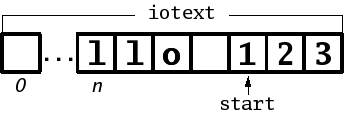
\includegraphics[scale=0.8]{Yytext1}
    \caption{\code{iotext} on entering an
      \code{FaAction}}\label{fig:iotextIn}
  \end{center}
\end{figure}

To perform the bracketing operation, the string \code{pre} is inserted
at \code{start} and \code{post} is appended to \code{iotext}. The
result is shown in figure~\ref{fig:iotextOut}.

\begin{figure}
  \begin{center}
    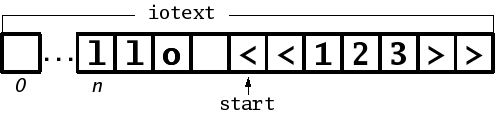
\includegraphics[scale=0.8]{Yytext2}
    \caption{\code{iotext} after adding \code{pre} and \code{post}}\label{fig:iotextOut}
  \end{center}
\end{figure}

This is all there is to it. A word is, however, necessary about the
content of \code{iotext} to the left of \code{start}. It contains text
that is already filtered but was not yet written to the output. Under
default conditions the action should not touch this text for the
simple reason that it may not be there. The lesson about collect mode
(section~\ref{sec:collect}) demonstrates how to use the flag
\hrefCollect to control exactly when processed text is written to the
output.

If you are not sure whether to implement an action in a file of its
own, as an embedded class or as an inner class,
section~\ref{sec:codeguide} about coding hints has a discussion
about it.


%%%%%%%%%%%%%%%%%%%%%%%%%%%%%%%%%%%%%%%%%%%%%%%%%%%%%%%%%%%%%%%%%%%%%%%%
\section{Co-operating Actions}\label{sec:coopActions}

Many applications of \monqjfa analyse input rather than filtering it.
No output text needs to be generated. Instead, information is
collected in a \code{HashMap} or in other objects.

Consider the task of counting how often each word appears in a
document. A \code{HashMap} shall be filled with the words as keys and the
counts as values. There are many ways to store the HashMap so that it
can be accessed within the action object, but the method described
here helps to keep the resulting \code{Dfa} shareable between parallel
threads. The lesson on thread safe \code{Dfa}
(section~\ref{sec:threadsafe}) describes why this is useful and
discusses why other implementations might fail.

Now it is time to download \hrefCountWords, which implements the task
described above. Compile it and check that it works:

\begin{codexa}
  \% echo hallo hallo bla bla bla | java CountWords\\
hallo: 2\\
bla: 3
\end{codexa}

The embedded class \code{DoCount} does the counting. The crucial lines
of its \code{invoke()} method read:

\begin{codexa}
  public void invoke(StringBuffer iotext, int start, DfaRun r) \{\\
  \T String word = iotext.substring(start);\\
  \T iotext.setLength(start);\\
     
  \T Map counts = (Map)r.clientData;\\
  \T ...\\
\}
\end{codexa}

First it fetches the word from \code{iotext} and then immediately
deletes it by trimming \code{iotext} to length \code{start}, because
no output needs to be produced. Then comes the access to the
\code{Map} that stores the word counts. The \code{Map} is found in the
\hrefClientdata field, which is specifically provided for such tasks.
But how did the \code{Map} object get there?

It is provided by the main method at the same time the DfaRun object
is created:

\begin{codexa}
  DfaRun r = new DfaRun(dfa);\\
  Map counts = new HashMap();\\
  r.clientData = counts;
\end{codexa}

Real applications usually need a bit more than just a \code{Map}
object in the \code{clientData} field and have to implement their own
class.  And typically there is more than one action object involved in
updating the data. But the general scheme is the same. When the
\code{DfaRun} object is created, the \code{clientData} field is also
set up, and then the actions update this object according to findings
in the text.

In principle you could store the \code{Map} as a field of
\code{DoCount}, but then this \code{Map} would be part of the
\code{Dfa} preventing it to be shared between different
threads. Section~\ref{sec:threadsafe} has more on this.




%%%%%%%%%%%%%%%%%%%%%%%%%%%%%%%%%%%%%%%%%%%%%%%%%%%%%%%%%%%%%%%%%%%%%%%%
\section{Collect Mode}\label{sec:collect}

Recall the signature of \hrefFaAction
\begin{codexa}
  public void invoke(StringBuffer iotext, int start, DfaRun r);
\end{codexa}

and the remark in the lesson on implementing actions
(section~\ref{sec:actions}) that the data in \code{iotext} before
\code{start} should not be touched, because it may not be there. This
data is the text that was handled by previous invocations of actions.
The variable \code{iotext} is used by the machinery as an output
buffer that is flushed at reasonable intervals. Hence the data is
there only if the buffer was not recently flushed.

Nevertheless there are situations where it is necessary to control the
times when \code{iotext} is flushed. As an example consider a search
for sentences that mention at least two protein names.  Rather then
assembling a convoluted regular expression to match exactly such
sentences, it is much easier to just match and count the protein
names. Reaching the end of the sentence, we delete it from
\code{iotext} if the count is less than 2. But how can we make sure
the sentence was not yet flushed to the output?

This is what \hrefCollect is for. As soon as it is set to \code{true}
the machinery will not drain \code{iotext} to the output anymore, and
filtered text is collected until \code{DfaRun.collect} is set to
\code{false} again. An outline to implement the protein-pair sentences
filter described above goes like this:

\begin{enumerate}
\item Write an action that sets \code{DfaRun.collect} to true at the
  start of the sentence and records the start in an object passed
  around between the actions via \code{r.clientData} (see
  section~\ref{sec:coopActions} on co-operating actions):
  \begin{codexa}
    public void invoke(StringBuffer iotext, int start, DfaRun r) \{\\
    \T Data d = (Data)r.clientData;\\
    \T d.start = start;  // record the start of the sentence\\
    \T d.count = 0;      // counts the number of protein names\\
    \T r.collect = true;\\
  \}
  \end{codexa}
\item Write an action to count your proteins. 
  \begin{codexa}
    public void invoke(StringBuffer iotext, int start, DfaRun r) \{\\
    \T Data d = (Data)r.clientData;\\
    \T d.count += 1;\\
  \}
  \end{codexa}
\item Write and action bound to the end of the sentence that either
  deletes or keeps the sentence. In any case, \code{DfaRun.collect}
  should be set to \code{false} again to allow for some output to be
  shipped.
  \begin{codexa}
    public void invoke(StringBuffer iotext, int start, DfaRun r) \{\\
    \T  Data d = (Data)r.clientData;\\
    \T if( d.count<2 ) \{\\
    \T\T iotext.setLength(d.start);  // this deletes the sentence\\
    \T \}\\
    \T r.collect = false;            // allow for some output\\
  \}
  \end{codexa}
\end{enumerate}

Apart from just deleting the sentence or let it pass through, you can
rewrite or annotate it in any way you want, as long as you don't touch
the data in \code{iotext} before \code{d.start}.


%%%%%%%%%%%%%%%%%%%%%%%%%%%%%%%%%%%%%%%%%%%%%%%%%%%%%%%%%%%%%%%%%%%%%%%%
\section{Thread Safe Dfa}\label{sec:threadsafe}

One of the major goals of writing Jfa was to allow for huge
\code{Dfa}. We regularly use more than 200000 regular expressions
encoding gene and protein names from
\hrefUniprot in slight spelling variations.
The result is a \code{Dfa} requiring $\approx$250MB of main memory.
Setting up and compiling the \code{Dfa} takes a few minutes.

Because it is comparatively slow to set up the \code{Dfa}, it makes
sense to put it into a server program that compiles the \code{Dfa}
once and then serves many invocations. And because the \code{Dfa}
requires a fair amount of memory, each thread of the server should
better use the same instance of the Dfa.

It is always safe to share a data structure between threads if it is
(treated) read-only. As far as \monqjfa has control over it, the
\hrefDfa is read-only. The changeable state necessary to keep track of
the progress of matching is stored in the \hrefDfaRun. Actions you
write yourself, however, are under your control alone. For an action
not to ruin the shareability of the \code{Dfa}, it must not have any
internal state that changes while the machinery is running.

A typical wrong example would be an action that uses a private field
to count occurences of matches. If the \code{Dfa} is then shared
between threads, two threads might be incrementing the count at the
same time. Section~\ref{sec:coopActions} on co-operating actions
describes a better approach.

A particularly hard to find mistake emerges if your action is an inner
class and you inadvertently use fields of the enclosing object. To
safeguard against it you may want to declare actions to be static
classes.

Section~\ref{sec:codeguide} discusses coding hints that proved
useful in many cases.

%%%%%%%%%%%%%%%%%%%%%%%%%%%%%%%%%%%%%%%%%%%%%%%%%%%%%%%%%%%%%%%%%%%%%%%%
\section{Actions From Scratch}\label{sec:actionFromScratch}

What could be the reason to implement an \hrefFaAction from scratch
instead of extending \hrefAbstractFaAction? This has to do with the
\hrefmergeWith method. It comes into play whenever two patterns 
have matches in common. Consider the following real life example.

An online resource like \hrefUniprot is used to automatically generate
a dictionary of proteins. To match protein names also at the start of
a sentence, the first character of the name must be matched case
insensitive. Consequently the protein name ``cox1'' is transformed
into the regular expression \code{[Cc]ox1}. You want good recall, so
the generalize even more and make the number at the end of the name
optional: \code{[Cc]ox[0-9]*}.

The idea is to match protein names in text and annotate them with the
database ID from \texttt{UniProt}. But where does
\code{FaAction.mergeWith} come into play? The problem is that the
resource contains many similar protein names. Another one could be
``cox'', which you generalize into \code{[Cc]ox}. Now you have two
patterns that both match the string ``cox'' and when the \code{Nfa} is
compiled, the machinery has to decide which action to trigger. You
learned in section~\ref{sec:confpats} on conflicting patterns that
this is resolved via a priority when using \code{AbstractFaAction}.
But selecting one of the actions is not the right approach here. You
rather would like to annotate a match with both IDs, the one for
``cox1'' as well as the one for ``cox''.

You could write some pretty heavy code to merge the patterns before
adding them to the \code{Nfa}, but that code is likely to replicate
what happens anyway during compilation of the \code{Nfa}. And here is
where \code{FaAction.mergeWith} comes into play. It is called whenever
two patterns are in conflict. The default implementation in
\code{AbstractFaAction} resolves the conflict through priorities. If
you implement \code{FaAction} yourself, you can follow other
strategies. In our protein example, you create a fresh action that
annotates with both IDs. For the details of how to do so, see
\hrefmergeWith and peek at the code of \code{AbstractFaAction}.

%%%%%%%%%%%%%%%%%%%%%%%%%%%%%%%%%%%%%%%%%%%%%%%%%%%%%%%%%%%%%%%%%%%%%%%%
\section{Coding Hints}\label{sec:codeguide}

After you have seen the bits and pieces of how to implement small
\code{Nfa/Dfa/DfaRun} combinations, you may wonder how to organize
your code in a non-trivial example. Below are a few hints which
proved helpful. Of course you may chose to do things
differently.

\subsection{static final Dfa}

As discussed in section~\ref{sec:threadsafe} on thread safe
\code{Dfa}, the \code{Dfa} is ideally a read only data structure. If,
in addition, it is designed to parse a single, fixed input format, it
is sufficient to have exactly only one instance of \code{Dfa} for that
input format. In such a case, declare

\begin{codexa}
  private static final Dfa dfa;
\end{codexa}

and use a \code{static} section to initialize it:

\begin{codexa}
  static \{\\
  \T try \{\\
  \T\T  Nfa nfa = new Nfa(...)\\
  \T\T\T    .or(...)\\
  \T\T\T    ...;\\
  \T\T  dfa = nfa.compile(...);\\
  \T\} catch( ReSyntaxException e ) \{\\
  \T\T  throw new Error("impossible", e);\\
  \T\} catch( CompileDfaException e ) \{\\
  \T\T  throw new Error("impossible", e);\\
  \T\}\\
\}
\end{codexa}

Make sure to include the \code{try}/\code{catch} block as shown. As
long as you are fiddling with the regular expressions during
development, these errors will be thrown, but once you got rid of
syntax errors and conflicting regular expressions, the exceptions will
never be thrown again.

To use the \code{Dfa}, you could just make it public. Another strategy
is to provide

\begin{codexa}
  public static DfaRun createRun() \{\\
  \T DfaRun result = new DfaRun(dfa);\\
  \T result.clientData = new MySpecialObject();\\
  \T return result;\\
\}
\end{codexa}

As explained in section~\ref{sec:coopActions} on co-operating actions,
collection of data from the parsed input should be done in an object
stored in \code{DfaRun.clientData}. The type of this object usually
matches specific requirements of the actions within the \code{Dfa} and
should therefore be provided when the \code{DfaRun} object is created.

\subsection{Dfa Wrapped}
If the \code{Dfa} is not completely determined, but rather depends on
parameters, a static method to create the automaton would be an
option. If, however, the actions in the \code{Dfa} need to find a
specific type of object in the \code{DfaRun.clientData} field, this
would leave it to the user of the \code{Dfa} to provide the object.

Instead of a static method, define a class that wraps the \code{Dfa}.
The constructor of the class should take the necessary parameters and
create the \code{Dfa} exactly once. In addition it should again have a
method called \code{createRun} to return a \code{DfaRun} for the
\code{Dfa} and initialize the \code{clientData} field as
necessary. Example code is shown in figure~\ref{fig:wrapit}.

\begin{figure}
\begin{codexa}
  public class Wrapit \{\\
  \T private final Dfa dfa;\\
  \T public Wrapit(String someRegexp)\\
  \T\T throws ReSyntaxException, CompileDfaException \{
\\
  \T\T Nfa nfa = new Nfa(...)\\
  \T\T\T .or(someRegexp, ...)\\
  \T\T\T ...;\\
  \T\T dfa = nfa.compile(...);\\
  \T\}\\
  \T public DfaRun createRun() \{\\
  \T\T DfaRun result = new DfaRun(dfa);\\
  \T\T result.clientData = new MySpecialObject();\\
  \T\T return result;\\
  \T \}\\
\}
\end{codexa}
\caption{Wrapping a \code{Dfa} that depends on a
  parameter.}\label{fig:wrapit}
\end{figure}

The structure of the code is similar to the previous case, except that
the scope holding the \code{Dfa} now is the wrapper object and not the
class itself. In addition we cannot catch the exception anymore,
because the regular expression provided to the constructor may produce
exceptions beyond our control.

\subsection{Action Writing}

When the automaton has many pattern/action pairs, a multitude of
action classes needs to be written. It surely is not necessary to put
them each into a separate file. In principle there are three ways to
easily code the usually small (in code size) classes for an action, as
shown in this example:

\begin{codexa}
  Nfa nfa = new Nfa(Nfa.NOTHING)\\
  \T .or("someregexp", new AbstractFaAction() \{\\
  \T\T\T public void invoke(StringBuffer iotext, int st, DfaRun r) \{\\
  \T\T\T\T // fiddle with iotext only\\
  \T\T\T \}\\
  \T\T \})\\
  \T .or("otherregexp", myAction)\\
  \T .or("Albert", new Append("Einstein"))\\
  \T .or("Niels", new Append("Bohr"))\\
  \T;
\end{codexa}

The first action is coded inline. With the exception of one- or
two-liners, this can easily become confusing. In addition, the
anonymous class is an inner class of the enclosing class despite the
fact that it is not necessary, not even desireable
(see section~\ref{sec:threadsafe}) for the code to be able to access
fields of the enclosing class.

The second form can be used instead for actions that do not need a
constructor with a parameter. Variable \code{myAction} is an
instance of an anonymous class:

\begin{codexa}
  private static final FaAction myAction = new AbstractFaAction() \{\\
  \T \dots\\
  \}
\end{codexa}

The third and fourth form should be used if the action has an obvious
need for a constructor with a parameter. For the well discussed
reasons (see section~\ref{sec:threadsafe}), the class should be declared
static and should not have a modifyable state:

\begin{codexa}
  private static class Append extends AbstractFaAction \{\\
  \T private final String s;\\
  \T public Append(String s) \{ this.s = s; \}\\
  \T ...\\
  \}
\end{codexa}


%%%%%%%%%%%%%%%%%%%%%%%%%%%%%%%%%%%%%%%%%%%%%%%%%%%%%%%%%%%%%%%%%%%%%%%%
\section{Key Features}\label{sec:keyfeatures}


\subsection{Pattern/Action Programming Model}
Performing different actions dependend on which regular expression
matches, requires a cascade of if-then-else statements when using
other regular expression engines, in particular \code{java.util.regexp}. In
contrast, \monqjfa allows to combine many pattern/action pairs
conceptually (and in fact internally) into one huge regular expression
which is matched all at once. The action bound to the matching pattern
is automatically called.

\subsection{Implicit Loop over Input Text}
There is no need write code to read input, perform a match and write
output. All this is taken care of by \monqjfa. You can concentrate on
the interesting part, i.e.{} pairing regular expressions with the
actions.

\subsection{Dfa vs.{} Nfa}
Many other widely used regular expression engines use so called
non-deterministic finite automata (NFA) internally to perform the
match. While this allows for some nifty features, it is slow because
the non-determinism must be simulated with a trial-and-error
backtracking approach. Whenever backtracking is necessary, the input
is read again to try another possibility. In contrast, monq.jfa uses
deterministic finite automata (DFA). Their key feature, determinism,
allows to perform the match by reading and inspecting each input
character exactly once. As a result, the speed of matching is mostly
independent of the number of regular expressions combined into the FA.

\subsection{Huge/Many Regular Expressions}
Several hundred thousand regular expressions can be handled at once.
Consequently a whole dictionary of words, possibly coding slight
spelling variations, can be put into the machinery.

\subsection{Capturing Subexpressions}
While this is a standard feature also in \texttt{java.util.regexp}, it
is unheard of for regular expression engines based on DFA.
\cite{Friedl02} even explains why this is impossible. While he is
right in the general case, \monqjfa provides a
\href{\urlCaptparen}{partial solution} that works for many practically
relevant cases.

\subsection{Shortest Match}
Newsgroups are full of messages showing confusion over how non-greedy
quantifiers really work. The major source of confusion seems to be
that people rather want a \href{\urlShortest}{shortest match}, a
feature uniquely available in \monqjfa.

%%%%%%%%%%%%%%%%%%%%%%%%%%%%%%%%%%%%%%%%%%%%%%%%%%%%%%%%%%%%%%%%%%%%%%%%
\section{Missing Features}

Some features are (still) missing from \monqjfa. Some of them are
nearly impossible to implement and will therefore not appear anytime
soon. Others are not to difficult to implement, but simply did not
make it yet into the code.

\subsection{Extended Character Classes}
Support for character classes based on \href{\urlUnicats}{UNICODE
  character properties} is not yet implemented. This makes it
cumbersome to specify for example the UNICODE letter character class.
It is planned to add this feature.

\subsection{Specialized Quantifiers}
None of the reluctant, greedy or posessive quantifiers of
\texttt{java.util.regexp} are provided. A feature that in part makes
up for this, is the shortest match as described above.

\subsection{Lookbehind and Lookahead}
These are not provided because they are nearly impossible to
implement correctly with deterministic finite automata (DFA).

\subsection{Backreferences}
These only work with non-deterministic finite automata (NFA), while
\monqjfa uses DFAs.

\subsection{Case Insensitive Matching}
Without looking to closely at it, I assume it can be implemented easily
as soon as I get serious requests for it.

\bibliographystyle{apalike}
\bibliography{citations}


\end{document}
